
\begin{figure}[!htb]
    \centering
    \begin{adjustbox}{minipage=\linewidth,scale=0.8}
    \Subfigure[0.48]{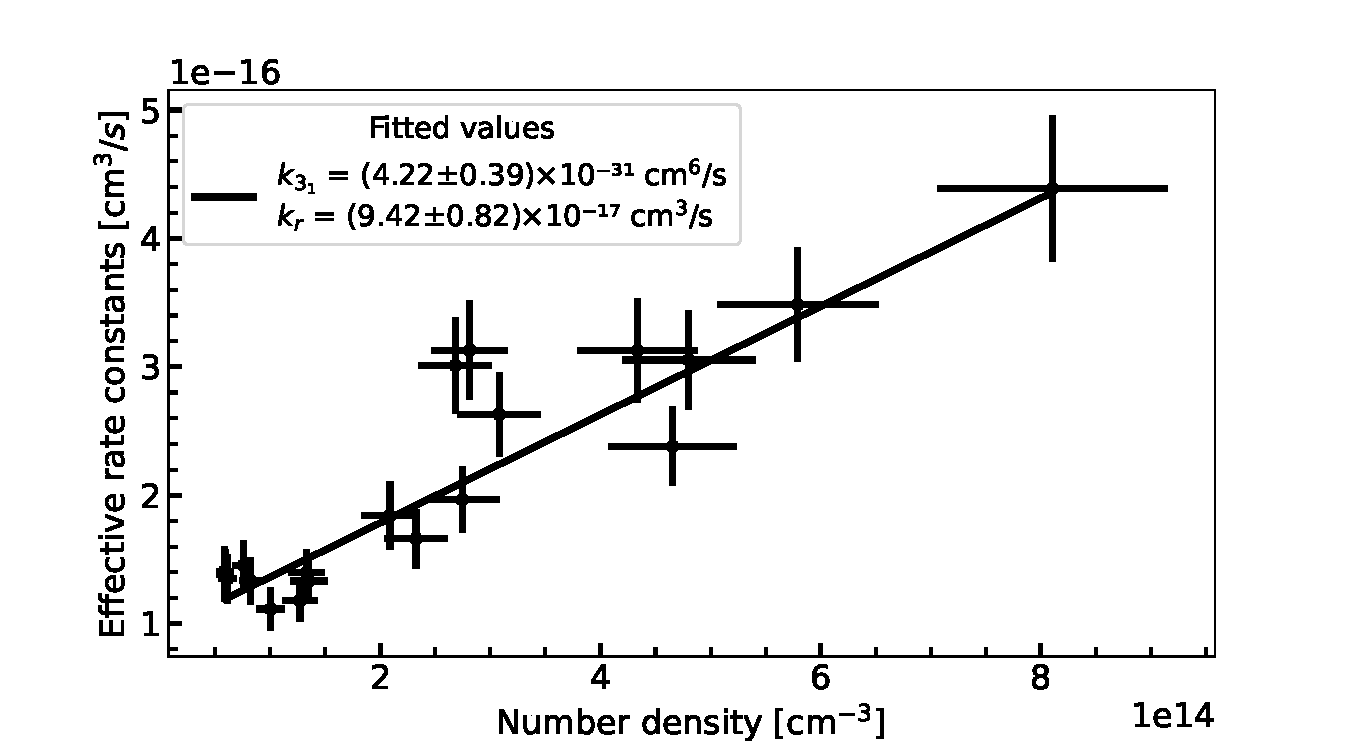
\includegraphics[width=1\textwidth]{figures/measurements/kinetics/functionOf_nHe/N+/off_4.7K_k31_effective_rate_constants.pdf}}{}{\label{fig:off:4.7k-effective-rate-constants:N+}}
    \hfill
    \Subfigure[0.48]{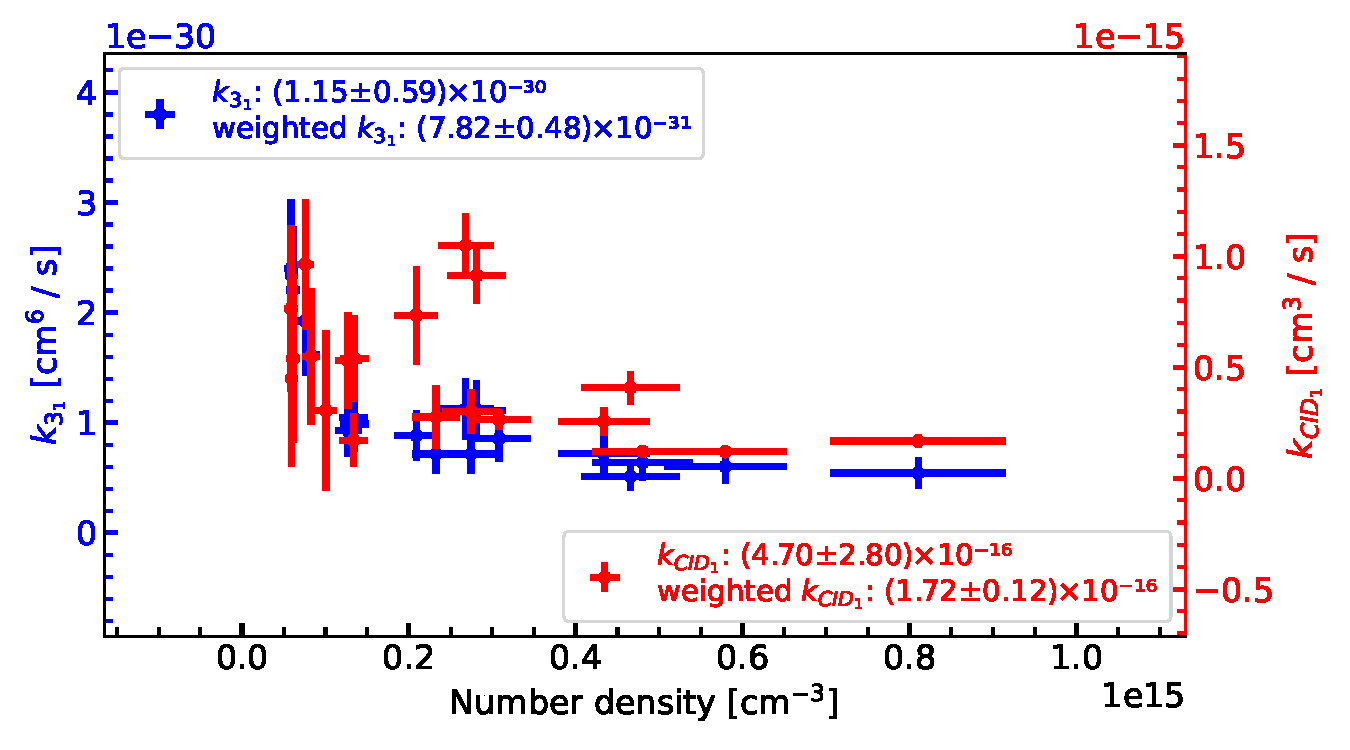
\includegraphics[width=1\textwidth]{figures/measurements/kinetics/functionOf_nHe/N+/off_4.7K_k3_kCID_1_as_functionOfnHe.pdf}}{}{\label{fig:off:4.7k-rate-constants:N+}}
    \hfill
    \Subfigure[0.48]{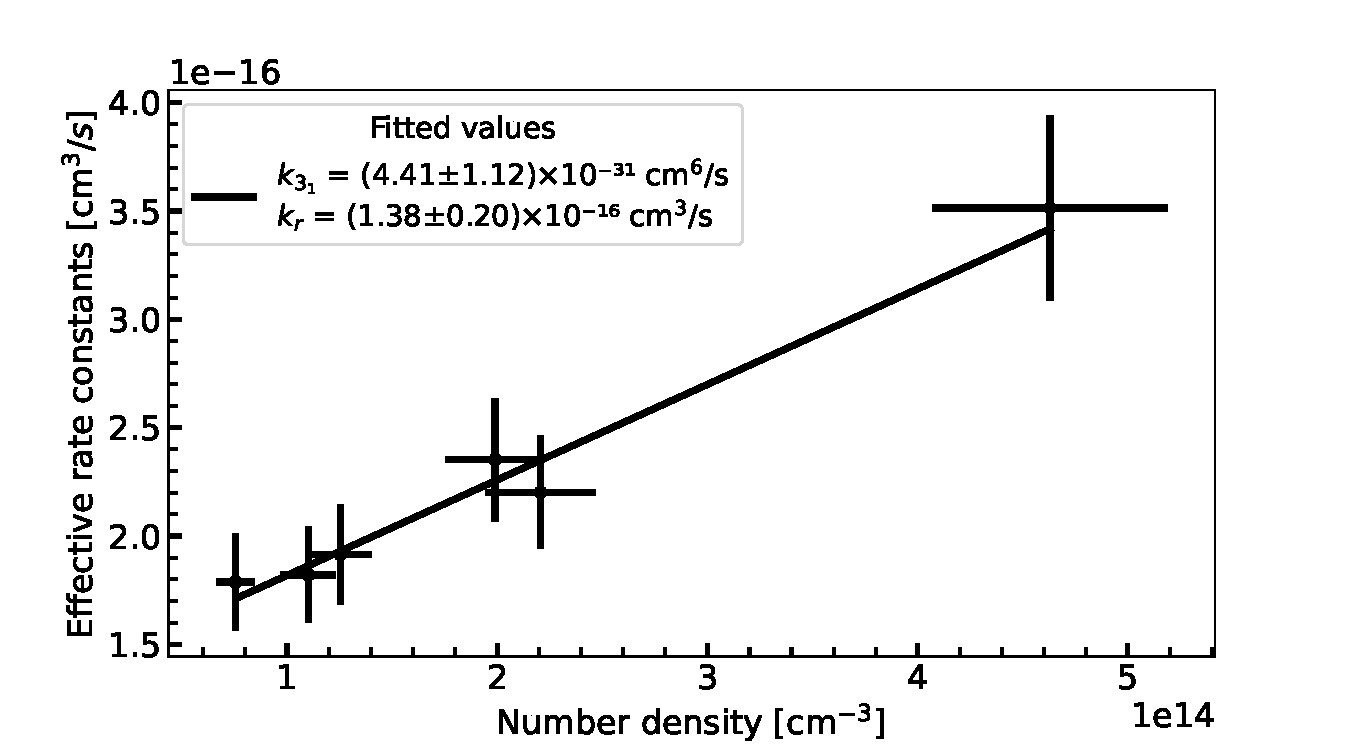
\includegraphics[width=1\textwidth]{figures/measurements/kinetics/functionOf_nHe/N+/off_6.5K_k31_effective_rate_constants.pdf}}{}{\label{fig:off:6.5k-effective-rate-constants:N+}}
    \hfill
    \Subfigure[0.48]{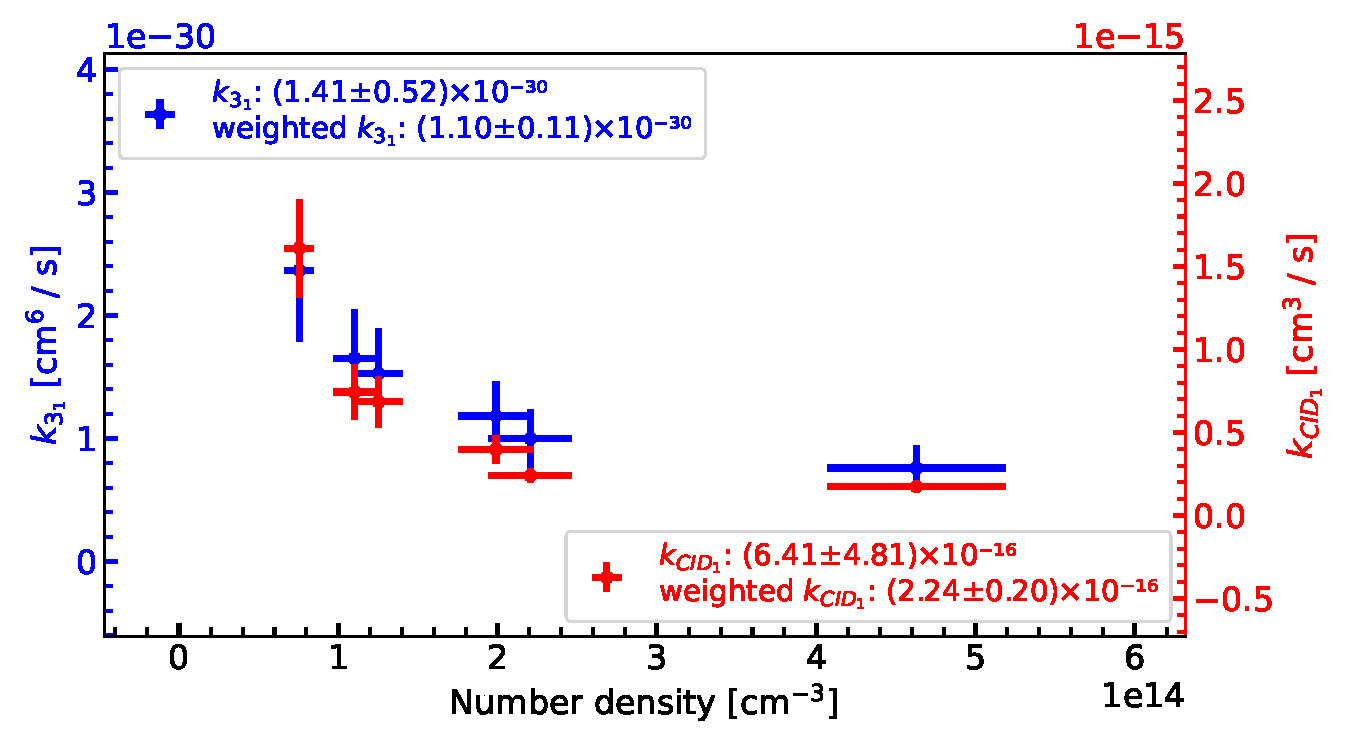
\includegraphics[width=1\textwidth]{figures/measurements/kinetics/functionOf_nHe/N+/off_6.5K_k3_kCID_1_as_functionOfnHe.pdf}}{}{\label{fig:off:6.5k-rate-constants:N+}}
    \hfill
    \Subfigure[0.48]{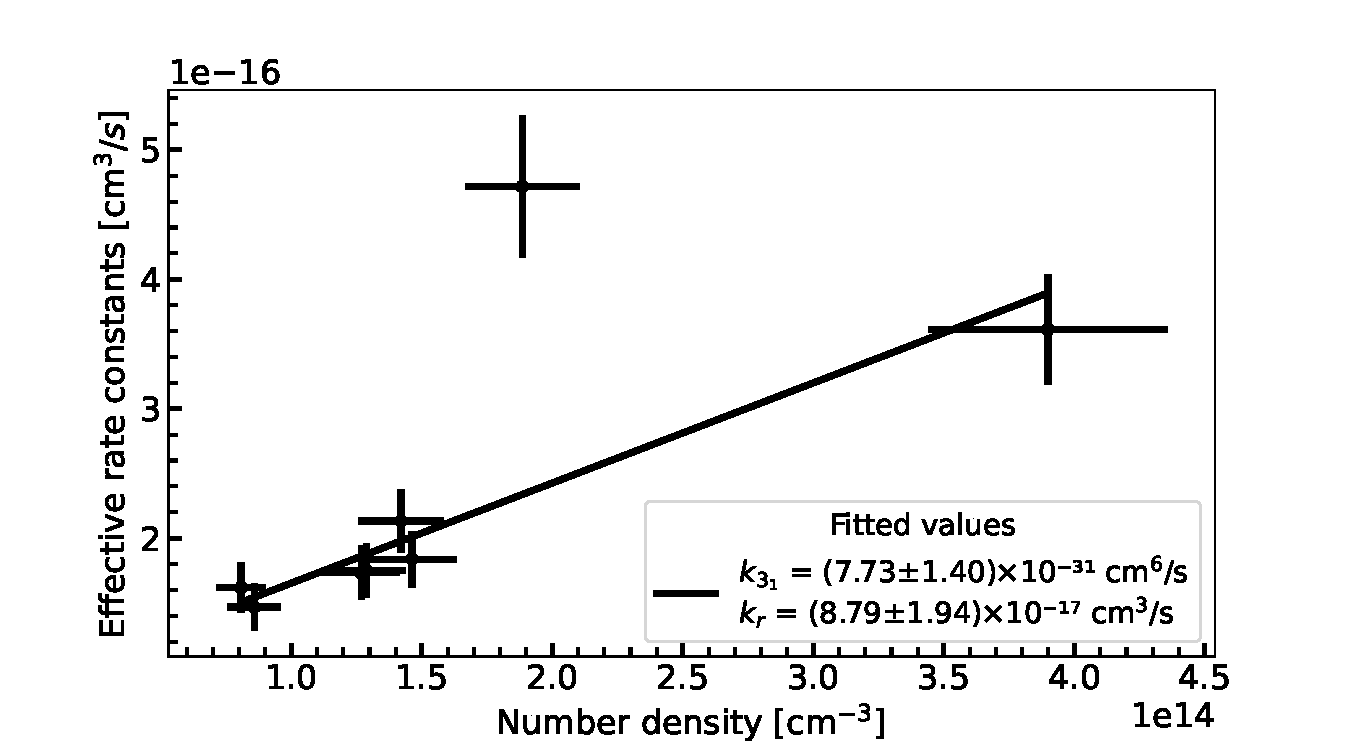
\includegraphics[width=1\textwidth]{figures/measurements/kinetics/functionOf_nHe/N+/off_8.4K_k31_effective_rate_constants.pdf}}{}{\label{fig:off:8.4k-effective-rate-constants:N+}}
    \hfill
    \Subfigure[0.48]{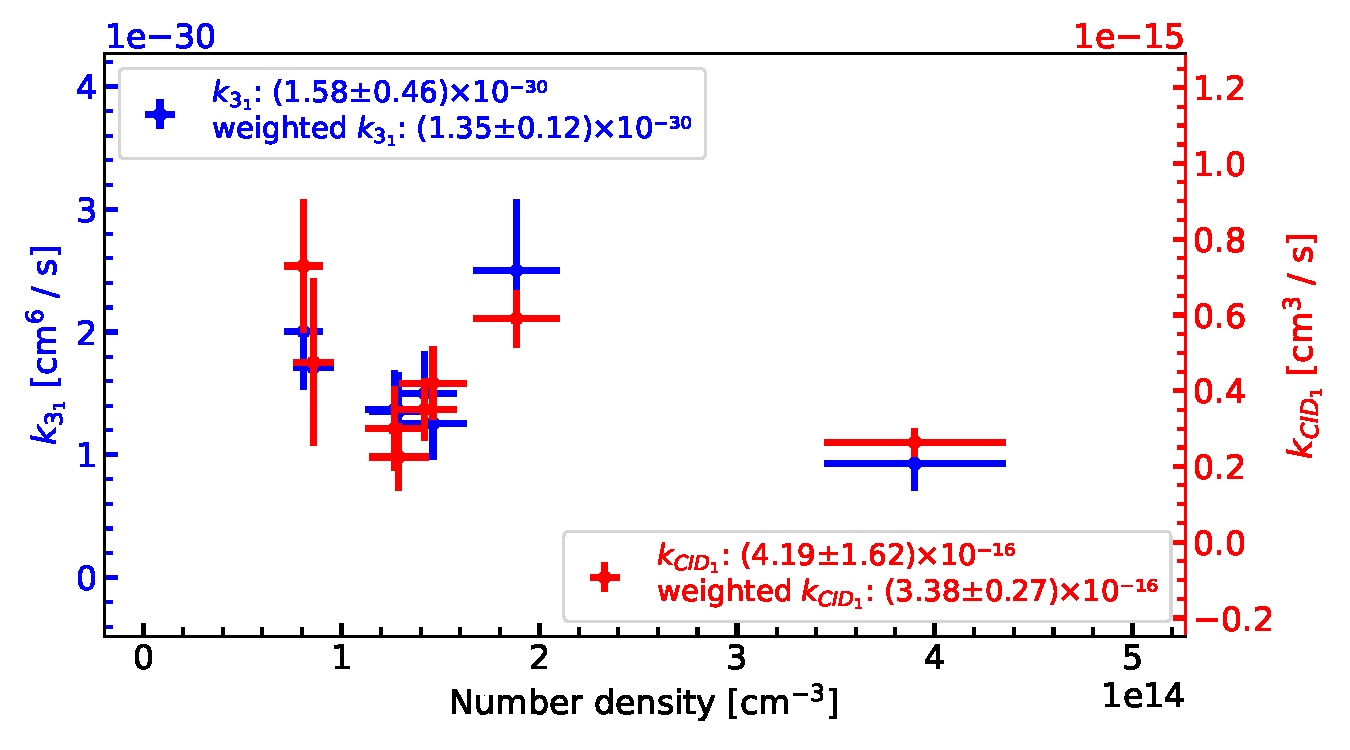
\includegraphics[width=1\textwidth]{figures/measurements/kinetics/functionOf_nHe/N+/off_8.4K_k3_kCID_1_as_functionOfnHe.pdf}}{}{\label{fig:off:8.4k-rate-constants:N+}}
    \hfill
    \Subfigure[0.48]{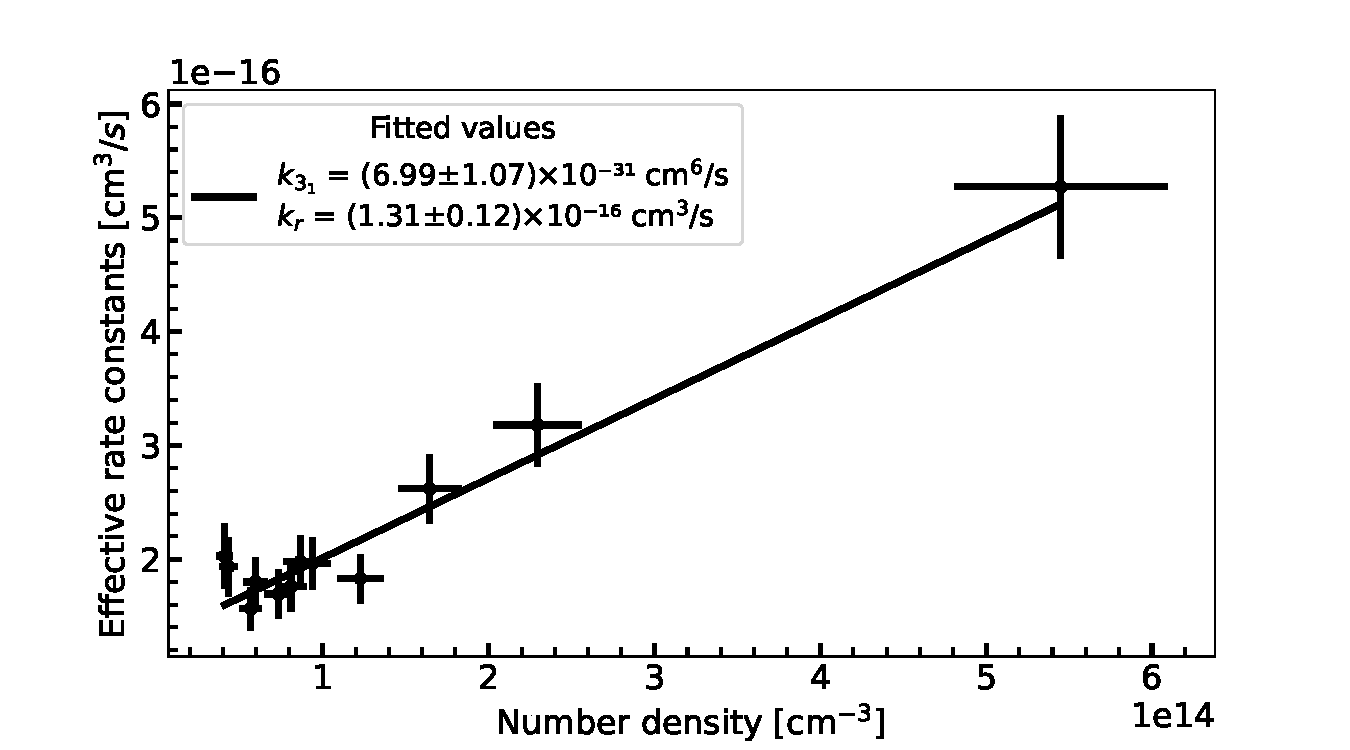
\includegraphics[width=1\textwidth]{figures/measurements/kinetics/functionOf_nHe/N+/off_10K_k31_effective_rate_constants.pdf}}{}{\label{fig:10k-off:effective-rate-constants:N+}}
    \hfill
    \Subfigure[0.48]{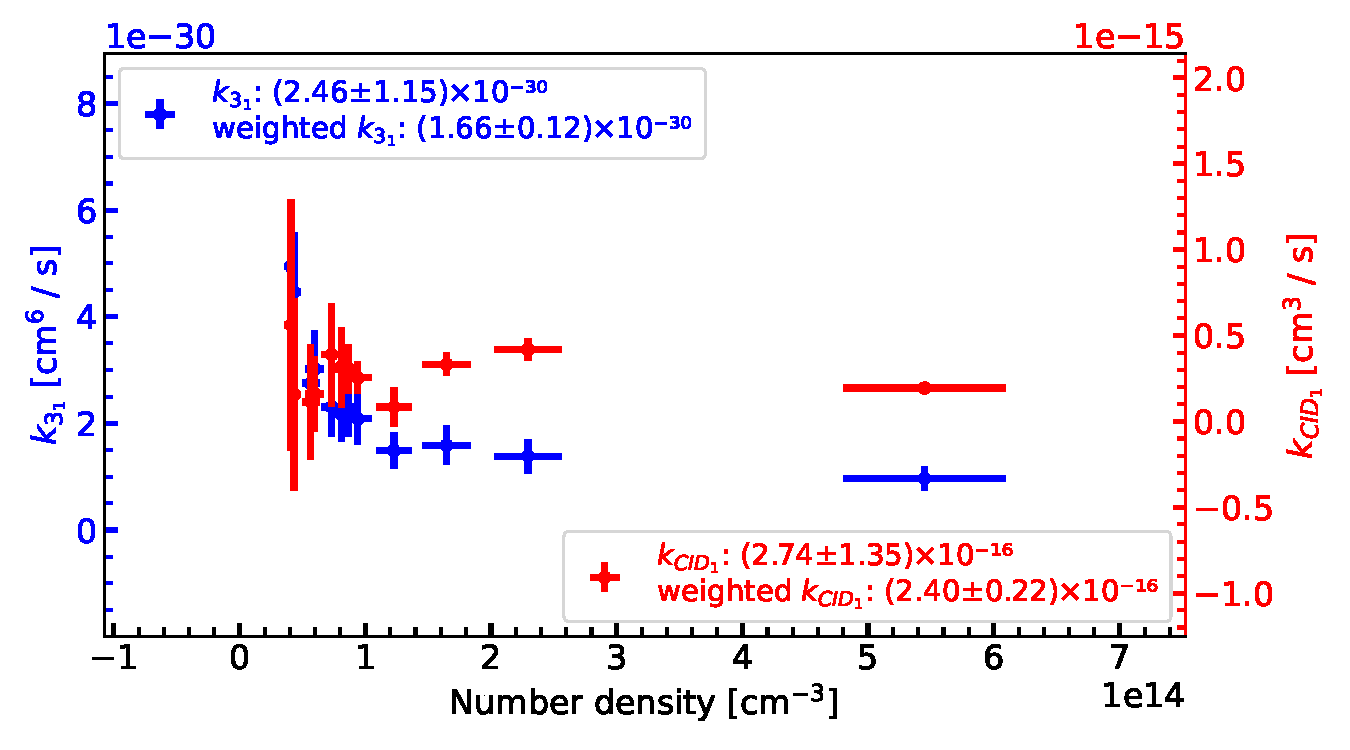
\includegraphics[width=1\textwidth]{figures/measurements/kinetics/functionOf_nHe/N+/off_10K_k3_kCID_1_as_functionOfnHe.pdf}}{}{\label{fig:off:10k-rate-constants:N+}}
    \hfill
    \end{adjustbox}
    \caption{
        N$^+$ + He reaction rate constants at $ (a) \& (b) \Rightarrow 4.8(3)$ K, $ (c) \& (d)\Rightarrow6.5(3)$ K, $ (e) \& (f)\Rightarrow8.4(3)$ K and $ (g) \& (h)\Rightarrow10.0(4)$ K: 
        The ternary association (\textcolor{blue}{$k_{3_1}$}) and collision-induced dissociation (\textcolor{red}{$k_{CID_1}$}) rate constants are plotted as a function of helium number density.
        (a, c, e, g) - represents: Effective binary rate constants are plotted as a function of number density to derive $k_{3_1}$ (ternary association) and $k_r$ (radiative) rate coefficients. 
        The solid line indicates the linear fit where the slope and intercept correspond to $k_3$ and $k_r$, respectively. 
        (b, d, f, h) corresponds to formation rate without $k_r$, the weighted average values are shown in the legend box (see Section \ref{subsec:rate-constants}).
    }
     \label{fig:rate-constants:N+}
\end{figure}